\documentclass[10pt,aspectratio=169]{beamer}
\usepackage[T1]{fontenc}
\usepackage[utf8]{inputenc}
\usepackage{lmodern}
\usepackage{amsmath,amssymb}
\usepackage{booktabs,array}
\usepackage{graphicx}
\usepackage{tikz}
\usetikzlibrary{arrows.meta,positioning}
\graphicspath{{figures/}}

\usetheme{default}
\definecolor{navy}{RGB}{31,78,156}
\definecolor{brick}{RGB}{192,57,43}
\definecolor{leaf}{RGB}{46,139,87}
\definecolor{figorange}{RGB}{230,126,34}
\setbeamercolor{structure}{fg=navy}
\setbeamercolor{title}{fg=navy}
\setbeamercolor{frametitle}{fg=navy}
\setbeamercolor{block title}{bg=navy!12,fg=navy}
\setbeamercolor{block body}{bg=navy!4}
\setbeamercolor{alerted text}{fg=brick}
\setbeamertemplate{navigation symbols}{}
\setbeamertemplate{footline}{\hfill\scriptsize\color{black!55}\insertframenumber/\inserttotalframenumber\hspace{2ex}\vspace{1ex}}
\setbeamertemplate{itemize items}[circle]
\setbeamertemplate{caption}{\scriptsize\insertcaption}
\setbeamerfont{frametitle}{size=\large,series=\bfseries}
\setlength{\leftmargini}{1.2em}
\setlength{\emergencystretch}{2em}
\newcommand{\code}[1]{\texttt{\detokenize{#1}}}
\newcommand{\1}{\mathbf{1}}
\newcommand{\R}{\mathbb{R}}
\newcommand{\E}{\mathbb{E}}
\newcommand{\Reg}{\mathrm{Reg}}
\newcommand{\W}{\mathcal{W}}
\DeclareMathOperator*{\argmax}{arg\,max}
\DeclareMathOperator*{\argmin}{arg\,min}
\newcommand{\good}[1]{\textcolor{leaf}{#1}}
\newcommand{\bad}[1]{\textcolor{brick}{#1}}

\title{The SPO portfolio tree: model v1}
\subtitle{What it is, how it is trained, and what the planted-threshold experiments say}
\author{Roman Beauvallet - Edo Theory}
\date{24 September 2026}

\begin{document}

\begin{frame}[plain]
\titlepage
\begin{center}\scriptsize\color{black!60}
Documents: \code{model_and_training_pipeline.tex} (the model), \code{experiments_planted_threshold.tex} and \code{experiments_regime_volatility.tex} (the experiments), \code{model_history.md} (the dated history). Main Code: \code{code/spo_tree.py}.
\end{center}
\end{frame}

% ---------------------------------------------------------------------------------------------------
\begin{frame}{The problem, and the bet}
\begin{columns}[T]
\column{0.55\textwidth}
\textbf{The problem.} Allocate between a few assets from a few features, every $h$ days, with fees, under noise and with 15 years of history: a \emph{decision} problem, not a forecasting one.

\medskip
\textbf{The bet} (\code{motivations.md}). A small tree that
\begin{itemize}
\item learns \emph{regimes} rather than a return manifold,
\item is trained on the \emph{decision regret} through the optimizer it feeds,
\item is judged on its own \emph{traded path}, fees included,
\end{itemize}
will be more stable, more implementable and interpretable than a larger predictor like a big DNN. 

\column{0.42\textwidth}
\begin{block}{What exists today}
\begin{itemize}
\item the tree and its exact optimizer, tested (64 unit tests);
\item a synthetic market with a \emph{planted} answer, so that recovery can be measured;
\item about 15{,}000 fitted trees over nine experiments (E1--E9);
\item a frozen configuration, \textbf{model v1}, validated on 100 datasets.
\end{itemize}
\end{block}
%\small Not yet: real data, decoy features at market-sized signals, the neural benchmark.
\end{columns}
\end{frame}

% ---------------------------------------------------------------------------------------------------
\begin{frame}{What the tree is, and what its nodes store}
\begin{columns}[T]
\column{0.57\textwidth}
\centering
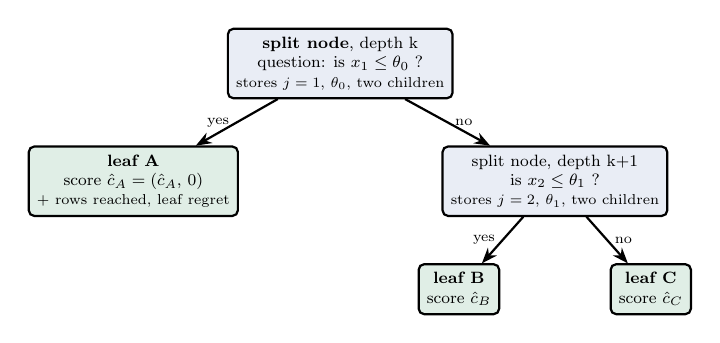
\begin{tikzpicture}[
  scale=0.74, every node/.style={transform shape, font=\footnotesize},
  split/.style={draw, thick, rounded corners=2pt, fill=navy!10, align=center, inner sep=4pt},
  leaf/.style={draw, thick, rounded corners=2pt, fill=leaf!15, align=center, inner sep=4pt},
  arr/.style={-{Stealth[length=2mm]}, thick}]
\node[split] (root) {\textbf{split node}, depth k\\ question: is $x_1\le\theta_0$ ?\\ {\scriptsize stores $j=1$, $\theta_0$, two children}};
\node[leaf, below left=0.8cm and -0.2cm of root] (A) {\textbf{leaf A}\\ score $\hat c_A=(\hat c_A,\,0)$\\ {\scriptsize + rows reached, leaf regret}};
\node[split, below right=0.8cm and -0.2cm of root] (S1) {split node, depth k+1\\ is $x_2\le\theta_1$ ?\\ {\scriptsize stores $j=2$, $\theta_1$, two children}};
\node[leaf, below left=0.8cm and -1.0cm of S1] (B) {\textbf{leaf B}\\ score $\hat c_B$};
\node[leaf, below right=0.8cm and -1.0cm of S1] (C) {\textbf{leaf C}\\ score $\hat c_C$};
\draw[arr] (root) -- node[left, font=\scriptsize] {yes} (A);
\draw[arr] (root) -- node[right, font=\scriptsize] {no} (S1);
\draw[arr] (S1) -- node[left, font=\scriptsize] {yes} (B);
\draw[arr] (S1) -- node[right, font=\scriptsize] {no} (C);
\end{tikzpicture}

\medskip
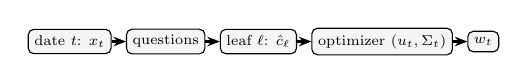
\begin{tikzpicture}[scale=0.74, every node/.style={transform shape, font=\scriptsize},
  box/.style={draw, rounded corners=2pt, inner sep=3pt, fill=black!4}, arr/.style={-{Stealth[length=1.6mm]}, thick}]
\node[box] (x) {date $t$: $x_t$};
\node[box, right=0.25cm of x] (route) {questions};
\node[box, right=0.25cm of route] (leaf) {leaf $\ell$: $\hat c_\ell$};
\node[box, right=0.25cm of leaf] (opt) {optimizer $(u_t,\Sigma_t)$};
\node[box, right=0.25cm of opt] (w) {$w_t$};
\draw[arr] (x) -- (route); \draw[arr] (route) -- (leaf); \draw[arr] (leaf) -- (opt); \draw[arr] (opt) -- (w);
\end{tikzpicture}

{\scriptsize How a date is used: answer the questions from the root down, read the leaf's score, let the optimizer turn it into weights from that date's holdings.}
\column{0.41\textwidth}
\footnotesize
\textbf{A tree} is a chain of yes/no questions on the features, ``is $x_j\le\theta$?'', ending in leaves. The root is the first question; a deeper split node is a question asked only of the rows that reached it; a leaf asks nothing.
\begin{itemize}
\item \textbf{A split node} (the root included) stores a feature index $j$, a threshold $\theta$ and its two children: yes goes left, no goes right. No score.
\item \textbf{A leaf} stores one score vector $\hat c_\ell$ (asset score, cash at 0), fed to the optimizer for every date that reaches it, plus the number of training rows it received and their leaf regret.
\item \textbf{Holdings, weights and returns belong to dates}, not to nodes: the tree stores no path.
\item Depth at most 3 (v1): at most 8 leaves, hence at most 8 scores. Growth turns one leaf into a split node with two new leaves, we add one leaf at each growth step; pruning does the reverse.
\end{itemize}
\end{columns}
\end{frame}
% ---------------------------------------------------------------------------------------------------
\begin{frame}{Notation}
\textbf{Notation}
\begin{itemize}
\item $r_t$ the realised $h$-day returns of the assets at decision $t$; cash has zero return.
\item $w_t\in\R^n$: the weights to be decided, including cash; $w\in\W$ (long-only, fully invested, cash included).
\item $u\in\R^n$: the weights held \emph{before} the decision, i.e.\ the previous portfolio after the drift of the period, $u_{t+1}=w_t\circ(1+r_t)/(1+r_t^\top w_t)$; $u_1=\1/n$.
\item $c\in\R^n$: the tree's scores, one per asset; cash has score $0$.
\item $\Sigma$: covariance of the $h$-day returns, from the past only: $h\times$ the covariance of the last 180 daily returns, plus $\varepsilon I$ ($\varepsilon=10^{-6}$); for the asset, $\sigma_h^2=h\,\hat\sigma^2$.
\item $f\in\R^n_{\ge0}$: fee per unit of traded notional (3 bp on the asset, 0 on cash)
\item $\lambda>0$: risk aversion (1 in v1)
\item $\bar w$: cap per asset (=1).
\end{itemize}
\end{frame}
% ---------------------------------------------------------------------------------------------------
\begin{frame}{The decision problem: notation and the exact solver}
\footnotesize
\textbf{The problem}, one decision every $h$ days over $n$ assets (here a coin and cash, $n=2$):
\[
w^\star(c;u,\Sigma)=\argmax_{w\in\W}\left(c^\top w -f^\top|w-u| - \lambda\,w^\top\Sigma w \right),
\quad \W=\{w\in\R^n:\ 0\le w_i\le\bar w,\ \textstyle\sum_iw_i=1\}
\]
Strictly concave ($\lambda>0$, $\Sigma\succ0$): one maximizer. Adding a constant to every score changes nothing (it only shifts the objective by a constant), since $1^\top w=1$: only score differences matter $\implies n-1$ degrees of freedom, feature is useful only if it shares relative returns information. \newline

\textbf{Exact solution by enumeration.} Lagrangian, with $\nu$ the multiplier of the budget: $L(w,\nu)=c^\top w-f^\top|w-u|-\lambda w^\top\Sigma w-\nu(\1^\top w-1)$. At the maximum each weight $w_i$ is in one of five states: at $0$; at $\bar w$; at $u_i$ (no trade in $i$: the fee kinks the objective there, so a whole range of scores leaves $w_i$ in place); strictly above $u_i$ (buying); strictly below $u_i$ (selling). In the last two the weight is \emph{free}: no bound and no kink pins it, so $\partial L/\partial w_i=0$ with the fee's sign known,
\[
c_i\mp f_i-2\lambda(\Sigma w)_i=\nu\quad\text{for every free asset } i,\qquad \partial L/\partial\nu=0 \iff \ \textstyle\sum_iw_i=1,
\]
so at the optimum all free assets share the same marginal net gain $\nu$. Fixing the state of every asset ($5^n$ cases) turns these equations into a linear system for the free weights and $\nu$. The solver takes the best objective among them: the optimum is found exactly, for all rows at once (\code{PortfolioOptimizer.solve}).
\end{frame}

% ---------------------------------------------------------------------------------------------------
\begin{frame}{Two assets: the exact solution in one line}
\small
Asset weight $w$, cash $1-w$ (cash: zero return, zero fee, variance $\approx0$). With $c$ the asset's score and $u$ its weight before the decision, the problem is one-dimensional:
\[
\max_{0\le w\le1}\ g(w)=c\,w-f\,|w-u|-\lambda\sigma_h^2\,w^2,\qquad \kappa:=2\lambda\sigma_h^2 .
\]
Away from the kink $g'(w)=c\mp f-\kappa w$ (minus when buying, $w>u$; plus when selling, $w<u$); at the kink, $u$ is optimal when $0$ lies between the two one-sided derivatives. Hence
\[
w^\star=\begin{cases}
\min\big\{\frac{c-f}{\kappa},\,1\big\} & \text{if } c-\kappa u>f \quad\text{(buy)}\\[5pt]
\max\big\{\frac{c+f}{\kappa},\,0\big\} & \text{if } c-\kappa u<-f \quad\text{(sell)}\\[5pt]
u & \text{if } |c-\kappa u|\le f \quad\text{(no trade)}.
\end{cases}
\]
\begin{columns}[T]
\column{0.47\textwidth}
\footnotesize
\textbf{Reading.} The fee-free target is $c/\kappa$: the position is linear in the score with slope $1/\kappa$, so all positions between 0 and 1 correspond to a score window of width $\kappa$ (from $c=f$ to $c=\kappa+f$ when buying from cash). The fee shifts the target by $f/\kappa$ towards the current holding and opens a no-trade band, $|c-\kappa u|\le f$ in score units, $f/\kappa$ in weight units.
\column{0.51\textwidth}
\footnotesize
\textbf{At v1's values} ($\lambda=1$, $\sigma=1\%$ a day, weekly, $f=3$ bp): $\sigma_h^2=5\times10^{-4}$ and $\kappa=10^{-3}$, so the position goes from 0 to 1 as the score goes from $0.03\%$ to $0.13\%$ a week. The tree's leaf scores are $\pm0.3$ to $0.5\%$ a week: \alert{positions are 0 or 1}, and the no-trade band ($0.3$ in weight units) hardly ever binds. With $\lambda=10$, $\kappa=1\%$ and the same scores give interior positions, the gradual profiles of Section~8. v1 keeps $\lambda=1$: at this stage the tree is a regime classifier, not a position sizer.
\end{columns}
\end{frame}

% ---------------------------------------------------------------------------------------------------
\begin{frame}{The loss: decision regret, not forecast error}
With the realised returns $r_t$ of decision $t$ and the holdings $u_t$ the tree really had,
\begin{align*}
U_t(w)&=r_t^\top w-f^\top|w-u_t|-\lambda\,w^\top\Sigma_t w,\\
\Reg_t(c)&=U_t\big(w^\star(r_t;u_t,\Sigma_t)\big)-U_t\big(w^\star(c;u_t,\Sigma_t)\big)\ \ge 0 .
\end{align*}
The regret is the utility lost by deciding on the scores $c$ instead of on the returns that happened, from the same holdings: the SPO loss of Elmachtoub \& Grigas with the fees and the risk term inside.

\medskip\small
\begin{columns}[T]
\column{0.48\textwidth}
\textbf{What the leaf learns.} The score vector of a leaf minimises the regret summed over its rows,
\[
\hat c_\ell=\argmin_{c\in[-b,b]^n}\ \sum_{t\in\ell}\Reg_t(c),\qquad b=10\%,
\]
by a bounded coordinate search (3 passes of 7 points per coordinate). The scores are not forecasts: they are whatever makes the optimizer take the right decision on the leaf's rows.
\column{0.48\textwidth}
\textbf{Three facts that shape everything.}
\begin{itemize}
\item Only differences of scores matter: $w^\star(c+\alpha\1)=w^\star(c)$; cash has score $0$.
\item The regret is measured on the holdings of the current tree, so fees are paid on real trades, not on rebalancing from scratch.
\item The regret uses the \emph{same} $\Sigma_t$ as the optimizer: a risk that the covariance estimate does not see cannot be learnt (slide~\ref{sl:regime}).
\end{itemize}
\end{columns}
\end{frame}

% ---------------------------------------------------------------------------------------------------
\begin{frame}{The tree, the path, and the two gates}
\small
\begin{columns}[T]
\column{0.5\textwidth}
\textbf{Tree.} Internal nodes split on one feature, $x_j\le\theta$; a leaf holds one score vector $\hat c_\ell$. A frozen tree is a map $x\mapsto\hat c(x)$, piecewise constant.

\medskip
\textbf{Path.} Scores are traded in time order from the initial holdings,
\begin{align*}
w_t&=w^\star(\hat c(x_t);u_t,\Sigma_t),\\
\pi_t&=r_t^\top w_t-f^\top|w_t-u_t|,\quad
u_{t+1}=\frac{w_t\circ(1+r_t)}{1+r_t^\top w_t},
\end{align*}
and the path's Sharpe ratio is $S=\mathrm{mean}(\pi)/\mathrm{std}(\pi)$ per decision ($0$ for an all-cash path). Fees are paid on real trades from drifted holdings.

\column{0.46\textwidth}
\textbf{Growth: two in-sample gates.} A candidate split is ranked by its regret reduction $\Delta=L_\ell(\hat c_\ell)-L_{\mathrm{left}}(\hat c_{\mathrm{left}})-L_{\mathrm{right}}(\hat c_{\mathrm{right}})$ and accepted only if the replayed Sharpe ratio of the whole tree rises.

\medskip
\textbf{Pruning: one out-of-sample judge.} The last 25\% of the training decisions never enter the growth. A split stays only if, there, it lowers the regret and raises the Sharpe ratio: a paired test on the checking rows, with a hurdle in standard errors (v1: 2 s.e., below the root only).

\medskip
\textbf{Then} every leaf is refitted on all training rows.
\end{columns}
\end{frame}

% ---------------------------------------------------------------------------------------------------
\begin{frame}{Training, step by step}
\begin{center}
\resizebox{0.9\textwidth}{!}{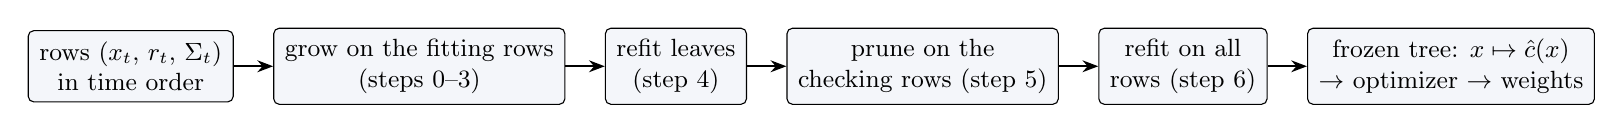
\begin{tikzpicture}[node distance=4mm and 5mm, every node/.style={font=\small},
  box/.style={draw, rounded corners=2pt, align=center, inner sep=4pt, fill=navy!5},
  arr/.style={-{Stealth[length=2mm]}, thick}]
\node[box] (rows) {rows $(x_t,\,r_t,\,\Sigma_t)$\\in time order};
\node[box, right=of rows] (grow) {grow on the fitting rows\\(steps 0--3)};
\node[box, right=of grow] (refit) {refit leaves\\(step 4)};
\node[box, right=of refit] (prune) {prune on the\\checking rows (step 5)};
\node[box, right=of prune] (final) {refit on all\\rows (step 6)};
\node[box, right=of final] (use) {frozen tree: $x\mapsto\hat c(x)$\\$\to$ optimizer $\to$ weights};
\draw[arr] (rows) -- (grow); \draw[arr] (grow) -- (refit); \draw[arr] (refit) -- (prune); \draw[arr] (prune) -- (final); \draw[arr] (final) -- (use);
\end{tikzpicture}}
\end{center}
\footnotesize
\begin{enumerate}
\item[0.] \textbf{Root.} One score vector on all fitting rows from equal holdings; replay it: holdings $u_t$, hindsight utilities, Sharpe $S$.
\item[1.] \textbf{Every leaf} of depth $<D$: refit it on the current holdings (yardstick); build the candidate thresholds (v1: deciles by rank among the admissible thresholds, then the neighbourhood of the best decile); screen each with a cheap regret $Q(\theta)$ (children scored by their clipped mean return); fit the children of the 3 best; keep a split if $\Delta/N_\ell>10^{-6}$.
\item[2.] \textbf{Choice.} Sort the kept splits of all leaves by $\Delta$; accept the first whose replayed Sharpe ratio beats $S$; none passes $\Rightarrow$ growth stops.
\item[3.] Replay the new tree: new holdings, utilities, $S$; back to step~1 (at most depth $D=3$, at least 20 decisions and 10\% of the parent per leaf).
\item[4.] \textbf{Refit} every leaf on the final holdings; kept if the Sharpe ratio does not fall.
\item[5.] \textbf{Prune} bottom-up on the checking rows: gain $g_t=\Reg_t(\text{without})-\Reg_t(\text{with})$; the split stays iff $\bar g>10^{-6}$, $\bar g>k_p\,\mathrm{se}(\bar g)$ and the checking Sharpe rises ($k_p=2$ below the root, $0$ at the root).
\item[6.] \textbf{Refit on all training rows}, rules fixed. The tree is frozen.
\end{enumerate}
\end{frame}

% ---------------------------------------------------------------------------------------------------
\begin{frame}{Model v1: the frozen configuration (24 September 2026)}
\scriptsize
\begin{tabular}{@{}p{2.2cm} p{4.4cm} p{6.8cm}@{}}
\toprule
Choice & v1 & Why (section of the experiments report) \\
\midrule
risk aversion $\lambda$ & 1 & positions 0/1; the tree is a regime classifier, sizing is not the object yet \\
fee & 3 bp on the asset, 0 on cash & market-sized; 10 bp starves the fast rates \\
decision rate & weekly ($h=5$); every 2 days as alternative & daily to weekly equivalent, monthly loses \\
depth & at most 3 & depth alone changes nothing if not reached\\
leaf minimum & 20 decisions and 10\% of the node & tail leaves at 0.7\% of the data \\
candidate thresholds & deciles by rank + local refinement (1 s.e.) & same Sharpe as the full screen, steadier thresholds \\
soft splits & \textbf{off} ($\kappa=0$) & never raise the Sharpe at $\lambda=1$ \\
growth gates & regret reduction, then the replayed Sharpe must rise & kept as designed; to be revisited in v2\\
pruning & last 25\% of the training decisions; hurdle 2 s.e. below the root, none at the root & the out-of-sample judge ; the hurdle removes spurious leaves at no cost \\
covariance & 180-day window, $\Sigma_t=h\,\hat\sigma_t^2$ & a 20-day window is noisier than it is timely (regime report)\\
conventions & cash column; all-cash Sharpe $=0$; $|\hat c|\le10\%$ & (7, model document)\\
\bottomrule
\end{tabular}

\smallskip
\textbf{In code:} \code{max_depth=3}, \code{min_samples_leaf=20}, \code{min_leaf_fraction=0.10}, \code{threshold_quantiles=deciles}, \code{refine_thresholds=True}, \code{refine_standard_errors=1}, \code{prune_standard_errors=2}, \code{prune_hurdle_from_depth=1}, \code{validation_fraction=0.25}, \code{fee_rate=(0.0003,0)}, \code{risk_aversion=1}: the setting \code{V1} of the experiments script. v1 is a \emph{configuration} of pipeline P4; every option it switches on is off by default, so the base of the experiments is P4 with everything off.
\end{frame}

% ---------------------------------------------------------------------------------------------------
\begin{frame}{The test-bed: a market with a planted answer}
\begin{columns}[T]
\column{0.54\textwidth}
\small One daily feature $x$ (Ornstein--Uhlenbeck) decides the regime of one asset:
\begin{gather*}
dx_t = k(m-x_t)dt + s\,dW_t\\
\frac{ds_t}{s_t} = \mu_t dt + \sigma_t dW_t,\quad \mu_t=\pm\mu\ \text{as}\ x_t\gtrless d,
\end{gather*}
with $\mu=e\,\sigma$, $e$ the \emph{edge} (daily drift over volatility).

\medskip\footnotesize
\begin{tabular}{@{}ll@{}}
\toprule
$\sigma$ & 1\% a day (16\% a year)\\
$e$ & 0.10, 0.05, 0.02 ($\pm25$, $\pm13$, $\pm5\%$ a year)\\
$k$ & 0.02 a day (half-life 35 days); 0.01 to 0.10\\
$m, s^2, d$ & 0, 1, 0: the threshold sits at the mean of $x$\\
$h$ & 1, 2, 5, 10, 21 days between decisions\\
data & 15 years of training, 5 of test, daily\\
\bottomrule
\end{tabular}

\column{0.44\textwidth}
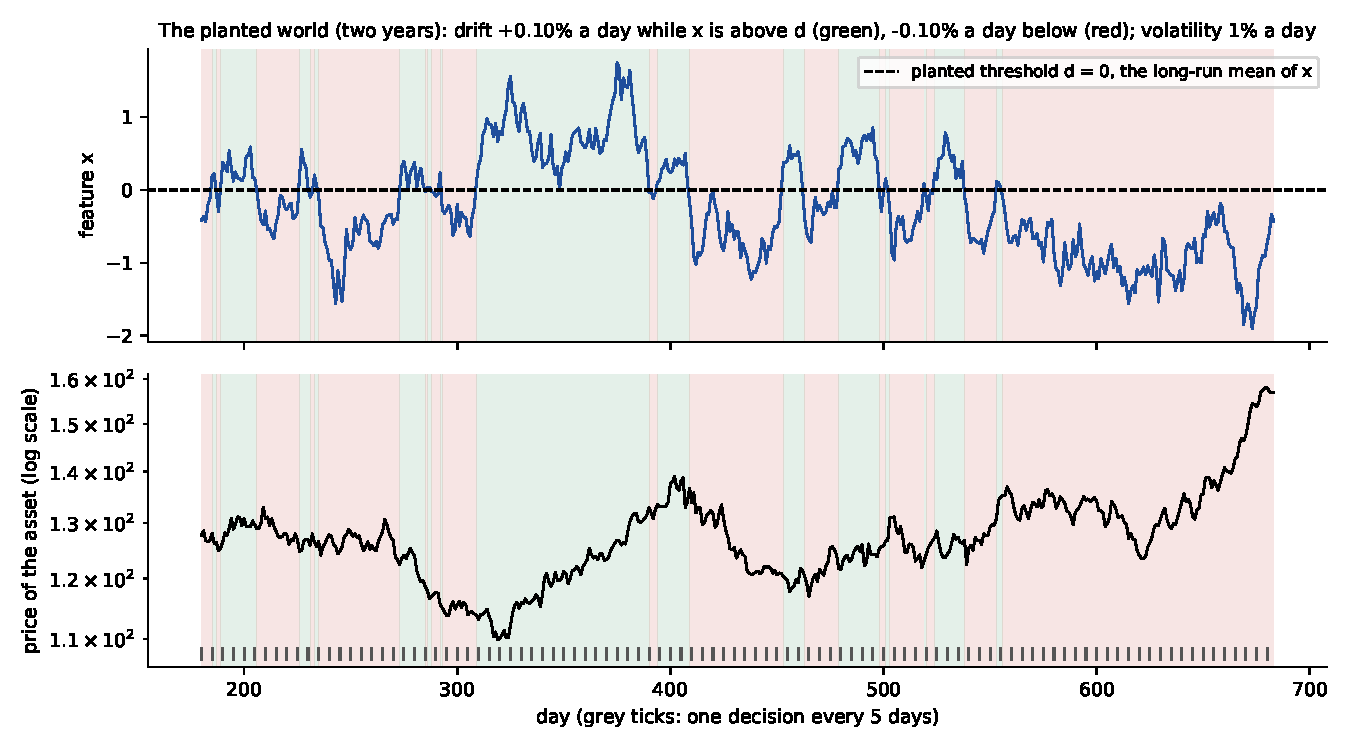
\includegraphics[width=\textwidth]{planted_world_one_dataset}
\footnotesize\textbf{What is measured}, over 40 to 100 datasets per cell: where the first threshold lands (target $d=0$, $x$ has standard deviation 1); the annualized test Sharpe ratio of the tree against the \emph{ideal rule} (the optimizer fed $\E[r\mid x]$: the best any method can do with $x$) and the \emph{rule at $d$}; the share of the ideal gain captured.
\end{columns}
\end{frame}

% ---------------------------------------------------------------------------------------------------
\begin{frame}{One fitted tree, read on its planted market (dataset 42, weekly, edge 0.10)}
\begin{columns}[T]
\column{0.54\textwidth}
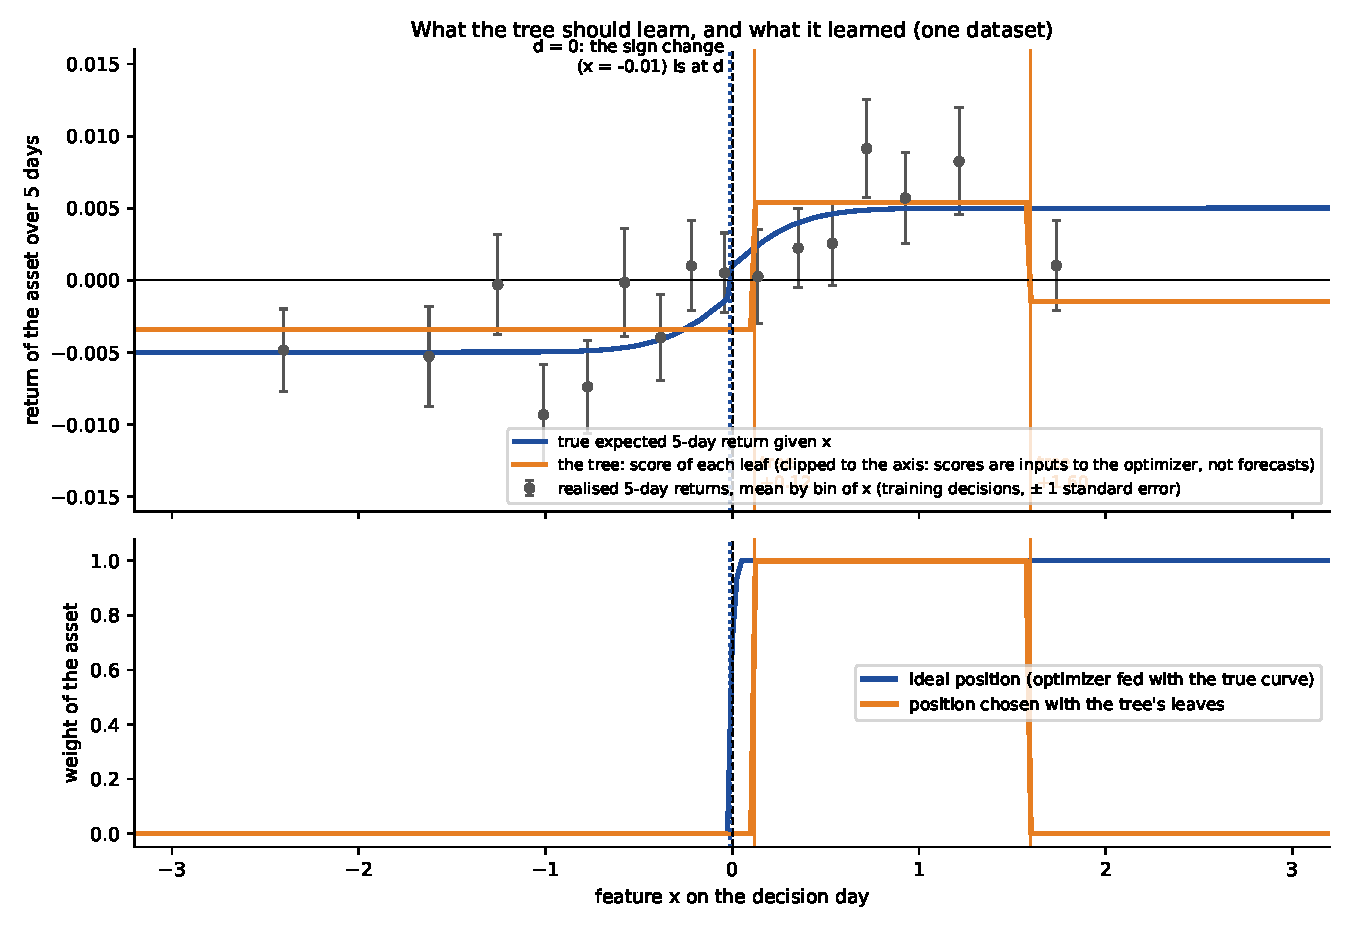
\includegraphics[width=\textwidth]{learned_vs_ideal_one_dataset}
\column{0.45\textwidth}
\scriptsize
\textbf{What is drawn} ($x$ on the decision day, horizontally).
\begin{itemize}
\item \textcolor{navy}{\textbf{blue curve}} (top): the true expected 5-day return given $x$, from the planted model; zero at $x=-0.01$, the planted $d=0$.
\item \textbf{grey dots}: realized 5-day returns of the training decisions, mean by bin of $x$ ($\pm1$ s.e.).
\item \textcolor{figorange}{\textbf{orange steps}} (top): the frozen tree's score, one level per leaf: $-0.35\%$ for $x\le0.12$, $+0.55\%$ up to $1.60$, $-0.15\%$ above.
\item \textbf{bottom}: the asset weight the optimizer chooses from a 50/50 portfolio when fed the blue curve (\textcolor{navy}{ideal rule}) or the tree's score (\textcolor{figorange}{tree}).
\end{itemize}
\textbf{Reading.}
\begin{itemize}
\item Root threshold $0.12$ for a planted $0$. The scores need not match the curve: both sit outside the $0.1\%$ window, so the position is 0 left of $0.12$ and 1 right of it, as the ideal rule's, up to $1.60$.
\item Above $1.60$ the base pipeline kept a leaf with a negative score: cash where the ideal rule stays invested. A few dozen decisions confirmed by a handful of checking rows; the v1 hurdle removes such leaves.
\item The ideal rule is a step too: at $\lambda=1$ the optimizer answers 0 or 1.
\end{itemize}
\end{columns}
\end{frame}

% ---------------------------------------------------------------------------------------------------
\begin{frame}{Result 1: the threshold is recovered at market sizes (E2, base pipeline)}
\begin{columns}[T]
\column{0.5\textwidth}
\scriptsize\setlength{\tabcolsep}{3pt}
\begin{tabular}{@{}rr r c rr r@{}}
\toprule
& & split & threshold & \multicolumn{2}{c}{annual.\ test Sharpe} & \\
\cmidrule(lr){5-6}
edge & $h$ & on $x$ (\%) & within 0.25 & tree & ideal & gain\\
\midrule
0.10 & 1 & 97 & 95\% & 0.80 & 1.03 & 76\%\\
 & 5 & 94 & 81\% & 0.73 & 0.88 & 79\%\\
 & 21 & 81 & 60\% & 0.54 & 0.68 & 75\%\\
\addlinespace
0.05 & 1 & 82 & 60\% & 0.12 & 0.49 & 25\%\\
 & 5 & 78 & 53\% & 0.24 & 0.43 & 51\%\\
 & 21 & 62 & 34\% & 0.17 & 0.35 & 43\%\\
\addlinespace
0.02 & 5 & 54 & 26\% & $-0.03$ & 0.15 & $-3\%$\\
\bottomrule
\end{tabular}

\smallskip\scriptsize
\textbf{How to read it.} One row = 100 datasets (50 at edge 0.02), each a fresh 15-year history with the threshold planted at $x=0$. \emph{$h$}: days between decisions. \emph{split on $x$}: share of the datasets whose tree keeps a split at all (with one feature, the alternative is no split). \emph{within 0.25}: share whose first threshold lies within 0.25 standard deviations of $x$ from the planted $0$. \emph{Sharpe}: annualized test Sharpe ratio, mean over the datasets (s.e.\ about 0.04); \emph{ideal} = the optimizer fed the true expected return given $x$. \emph{gain}: the tree's test return above the tree without splits, as a share of the ideal rule's.
\column{0.48\textwidth}
\footnotesize
\textbf{What the table says.}
\begin{itemize}
\item \textbf{With a drift of $\pm25\%$ a year the threshold is found at every rate.} Almost every tree splits, most thresholds land within 0.25 of the planted 0, and the tree earns 75 to 79\% of the ideal rule's gain out of sample.
\item \textbf{With $\pm13\%$ it degrades gracefully.} Fewer trees split, the threshold is less precise, and the tree captures 25 to 51\% of a gain that is itself small (ideal Sharpe 0.35 to 0.49).
\item \textbf{With $\pm5\%$ there is nothing to find in 15 years.} Half of the trees keep no split, the other half split at random ; the tree's Sharpe is 0 and the ideal rule's nearly so (0.15). Finding nothing is the right answer.
\item \textbf{Rate:} daily to weekly are equivalent; monthly loses precision and Sharpe, because a decision is held while the regime changes.
\end{itemize}
\end{columns}
\end{frame}

% ---------------------------------------------------------------------------------------------------
\begin{frame}{Result 2: the trading rate against the speed of the feature (edge 0.10)}
\begin{columns}[T]
\column{0.5\textwidth}
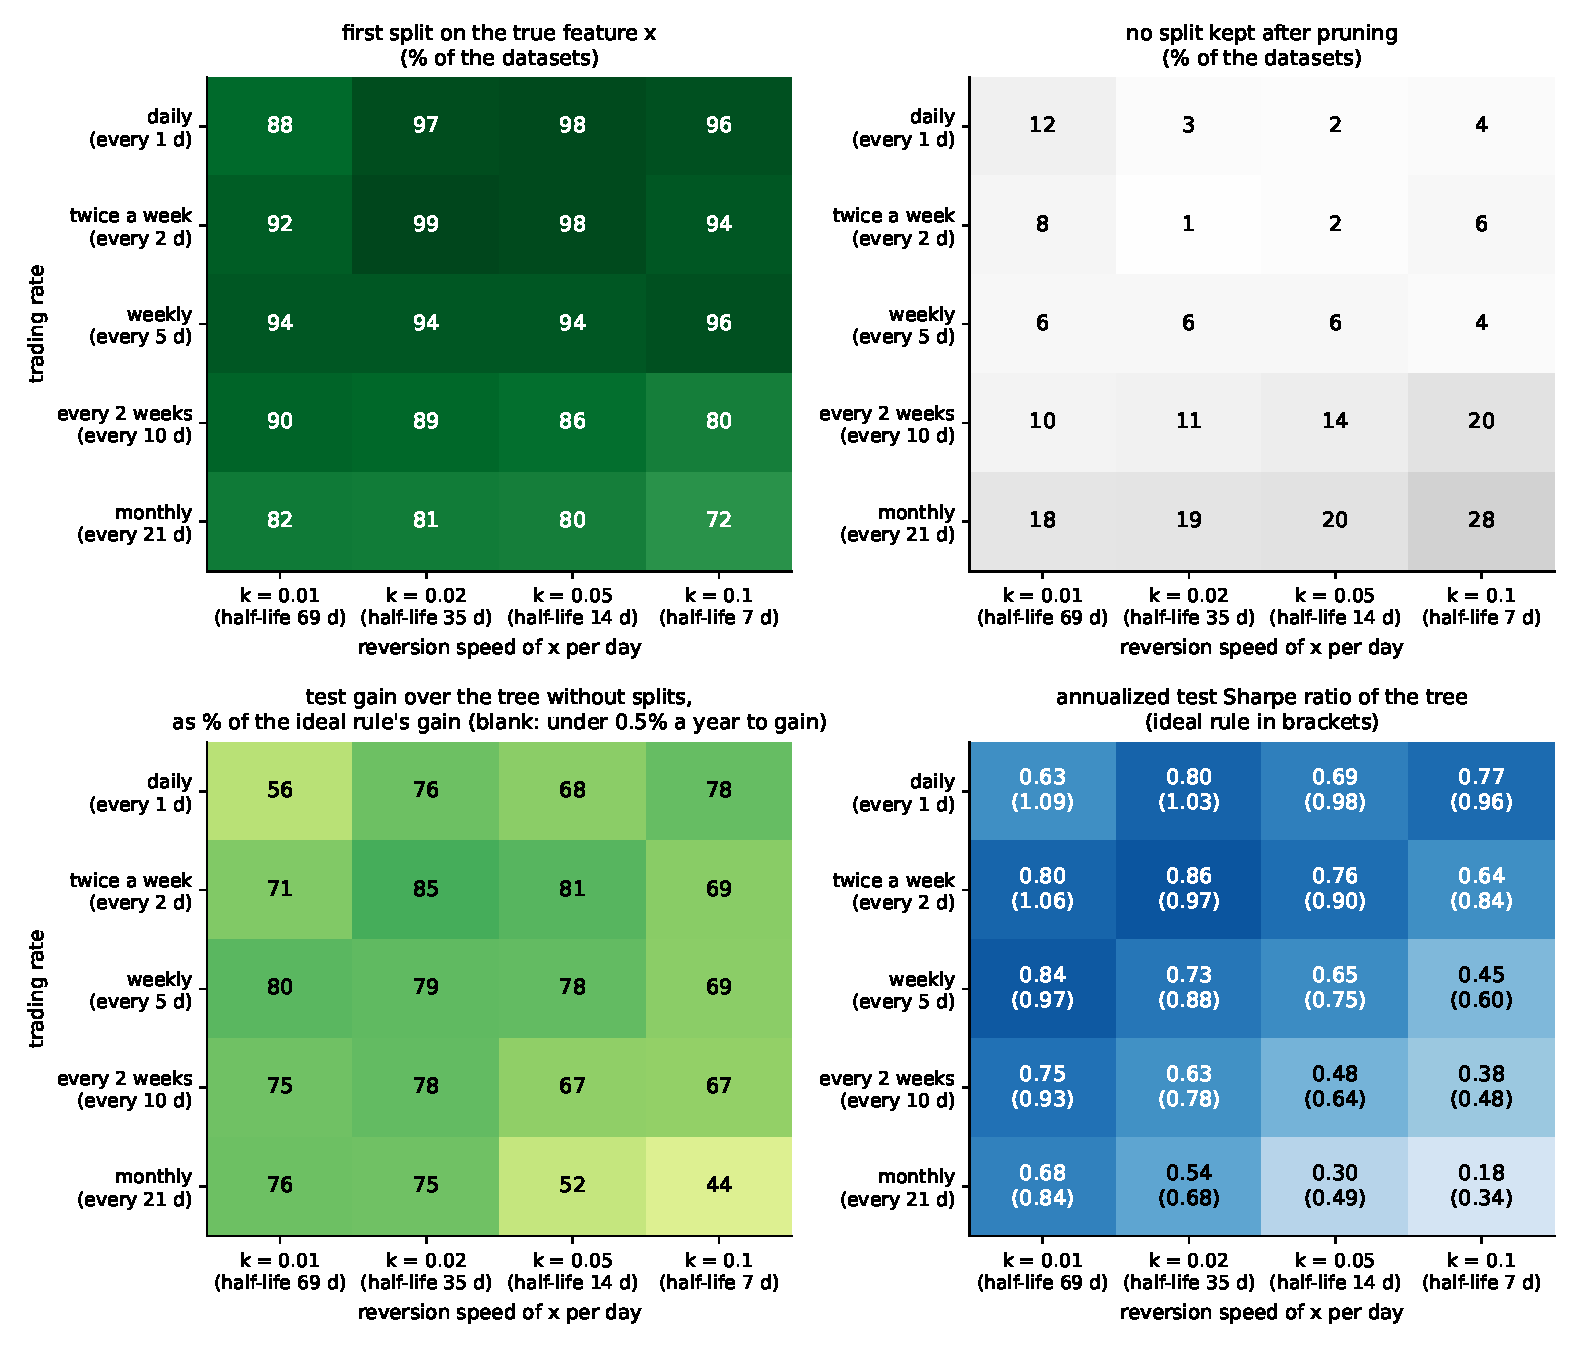
\includegraphics[width=\textwidth]{maps_rate_vs_speed}
\column{0.48\textwidth}
\small
\begin{itemize}
\item Daily to weekly decisions are equivalent: deciding more often than the feature moves adds fees, not information.
\item Monthly decisions lose precision and profit, the more so when the feature is fast: with a half-life of 7 days the tree's Sharpe is 0.77 daily and 0.18 monthly (ideal rule 0.96 and 0.34); the regime flips inside the holding period.
\item With a slow feature (half-life 69 days) the daily tree under-performs (0.63 against 1.09): 3{,}780 decisions on a signal that hardly moves make the tree over-trade its own noise.
\item Hence \textbf{weekly} in v1, with every 2 days as the alternative.
\end{itemize}
\end{columns}
\end{frame}

% ---------------------------------------------------------------------------------------------------
\begin{frame}{Risk aversion, fees and depth (E3, 1{,}920 fits): why v1 keeps $\lambda=1$}
\begin{columns}[T]
\column{0.4\textwidth}
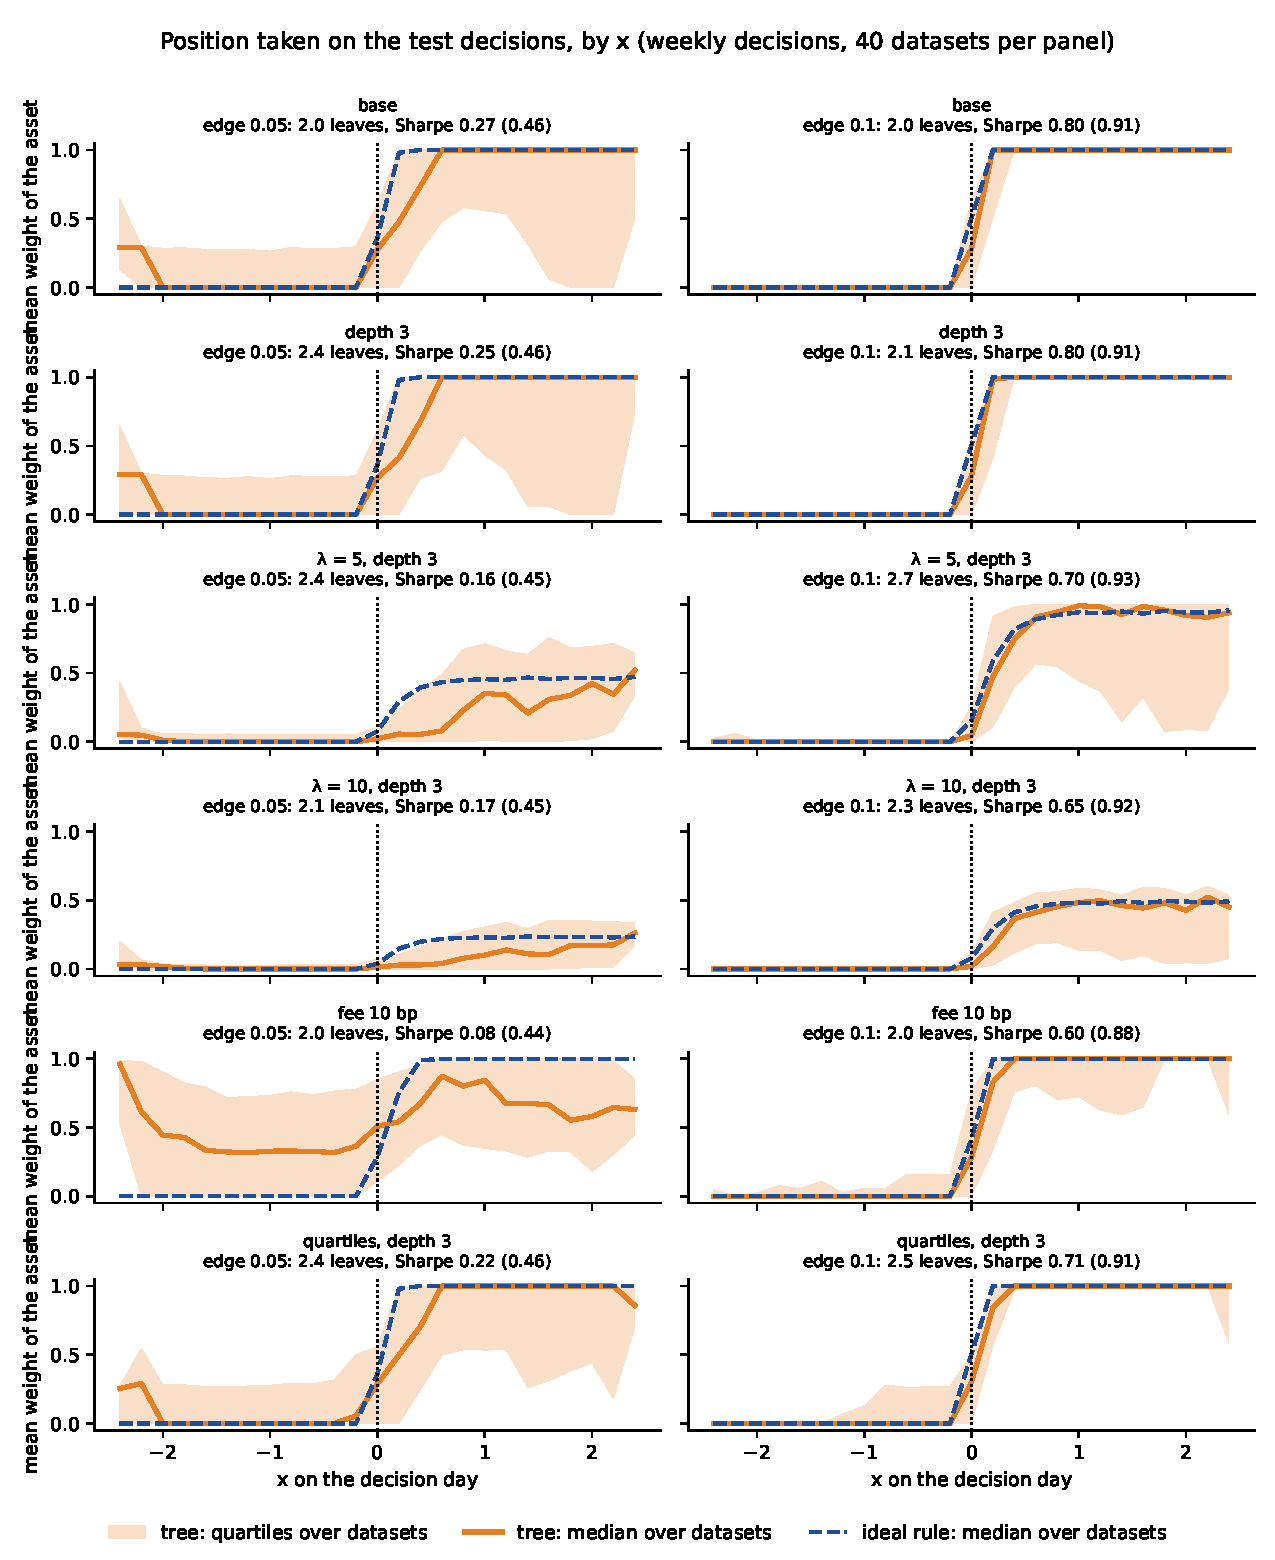
\includegraphics[width=\textwidth]{risk_fee_depth_positions}
\column{0.58\textwidth}
\small
Mean position of the asset by bin of $x$ on the test decisions, weekly, edge 0.10, against the ideal rule on the same information.
\begin{itemize}
\item \textbf{$\lambda=5$ and 10 make the positions gradual}, and the tree learns them, at a cost of 0.1 to 0.15 of Sharpe (0.70 and 0.65 against 0.80 weekly).
\item \textbf{A 10 bp fee} keeps positions at 0/1 and starves the fast rates: 0.53 against 0.88 every 2 days, turnover halved.
\item \textbf{Values' quartiles as the only candidates} lose at the fast rates (0.64 against 0.88 every 2 days).
\end{itemize}
Decision for v1: $\lambda=1$, 3 bp, depth at most 3. Sizing is a later question (at $\lambda=10$ the tree does size as the ideal rule does).
\end{columns}
\end{frame}

% ---------------------------------------------------------------------------------------------------
\begin{frame}{Split-search options: quantile candidates, refinement, soft splits}
\scriptsize
At a leaf with rows $I$ ($N$ rows) a child must keep $m_\ast=\max(m,\lceil\varphi N\rceil)$ rows ($m=20$, $\varphi=10\%$ in v1). The \textbf{plain} candidates of a feature are the midpoints between consecutive distinct values, $\theta_{(1)}<\dots<\theta_{(K)}$, whose two sides both keep $m_\ast$ rows. Each candidate is \textbf{screened} cheaply, each child getting its clipped mean return as score:
\[
Q(\theta)=\sum_{t\in I}\Reg_t\big(c_{\mathrm{side}(t)}(\theta)\big),\qquad
c_{\mathrm{left}}(\theta)=\mathrm{clip}\Big(\mathrm{mean}\{r_t:\ x_t\le\theta\},\ \pm b\Big),\ \text{likewise on the right.}
\]
\begin{columns}[T]
\column{0.5\textwidth}
\textbf{Quantile candidates + refinement} (on in v1)
\begin{itemize}
\item \emph{Deciles by rank.} Instead of all $K$ candidates, keep the nine at ranks $\mathrm{round}(q\,(K-1))$, $q=0.1,\dots,0.9$: evenly spread over the admissible range, never on its edge. The full screen costs $K\approx N-2m_\ast$ solves, this costs 9.
\item \emph{Refinement.} Let $\theta_\circ$ be the best decile. Screen every plain candidate strictly between its two neighbouring deciles; let $\theta_\bullet$ be the best of them. It replaces $\theta_\circ$ only if the improvement is clear,
\[
Q(\theta_\circ)-Q(\theta_\bullet)>k\cdot\mathrm{se},\qquad \mathrm{se}=\sqrt{|I|}\;\mathrm{std}_t(\delta_t),
\]
$\delta_t$ the per-row difference of the two regrets, $k=1$ in v1. The 3 best survivors get the full fit of their children.
\end{itemize}
\column{0.48\textwidth}
\textbf{Soft split} (off in v1: $\kappa=0$)
\begin{itemize}
\item Keep \emph{all} candidates $\theta_1<\dots<\theta_K$ of the feature, with Boltzmann weights from their screened regrets:
\[
z_k=\frac{Q(\theta_k)-\min_lQ(\theta_l)}{\mathrm{se}_k},\qquad
\pi_k=\frac{e^{-z_k/\kappa}}{\sum_le^{-z_l/\kappa}}
\]
(Gaussian variant $e^{-z^2/2\kappa^2}$): thresholds the data cannot tell from the best share the weight, clearly worse ones get none.
\item A row with value $x$ goes left with weight $\mu(x)=\sum_{k:\,\theta_k\ge x}\pi_k$, right with $1-\mu(x)$; weights multiply down the tree ($\omega_{t\ell}$), the leaf fit minimises $\sum_t\omega_{t\ell}\Reg_t(c)$, and a row's score is the mixture $\hat c(x_t)=\sum_\ell\omega_{t\ell}\hat c_\ell$: a ramp in $x$ instead of a jump. As $\kappa\to0$ the plain split is recovered.
\end{itemize}
\end{columns}
\end{frame}

% ---------------------------------------------------------------------------------------------------
\begin{frame}{Options tried, 1: candidate thresholds and soft splits (E4, E8; 3{,}840 fits)}
\begin{columns}[T]
\column{0.36\textwidth}
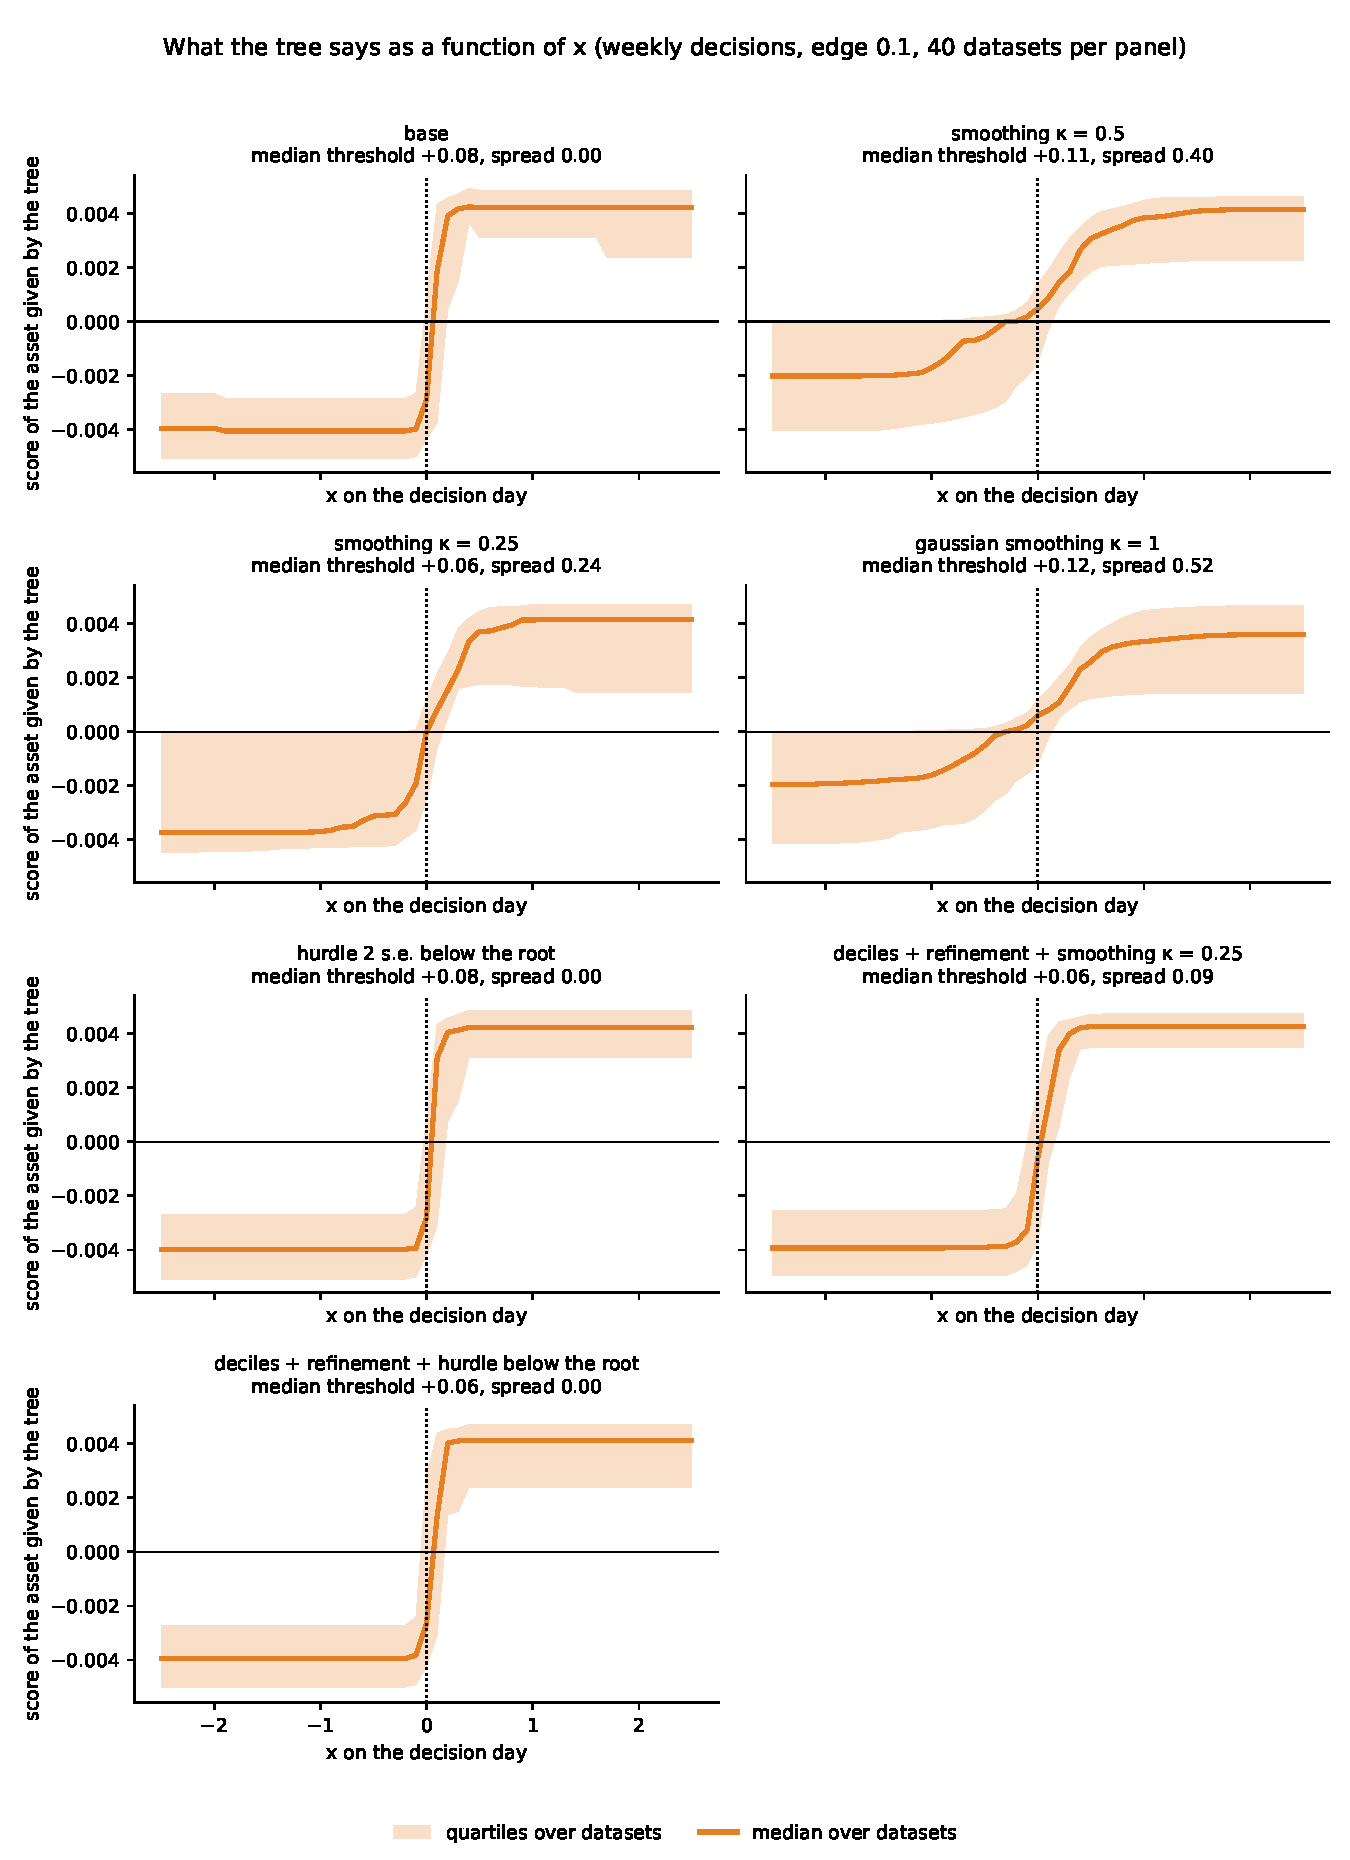
\includegraphics[height=0.8\textheight]{split_options_2_scores}
\column{0.62\textwidth}
\footnotesize
The tree's score as a function of $x$, weekly, edge 0.10 (median and quartiles over 40 datasets).
\begin{itemize}
\item \good{\textbf{Deciles by rank + local refinement}} (in v1): screen the deciles of the admissible thresholds, then the neighbourhood of the best one. Sharpe 0.82 against 0.80 for the base weekly; thresholds steadier at the slow rates (within 0.25 of $d$ monthly: 57\% against 45\%); ten times fewer candidates. It buys stability, not Sharpe.
\item \bad{\textbf{Soft splits}} (Boltzmann weights over the candidates; off in v1): at $\kappa=1$ the transition is 0.65 wide and the averaged score falls in the optimizer's no-trade band, so the tree stops trading (0.53 against 0.80 weekly, 0.35 against 0.87 every 2 days). At $\kappa=0.25$ the spread falls to 0.2 and the tree matches the base from weekly on, but still loses 0.26 every 2 days. On top of deciles and refinement it gives the narrowest transition (0.1) and the best weekly numbers (0.82, 85\% of the gain), within noise of the base.
\item Verdict: at $\lambda=1$ smoothing the score does not size the position; the option stays in the code for $\lambda\ge5$.
\end{itemize}
\end{columns}
\end{frame}

% ---------------------------------------------------------------------------------------------------
\begin{frame}{Options tried, 2: a calibrated pruning hurdle (E5, E8; 3{,}840 fits)}
\begin{columns}[T]
\column{0.42\textwidth}
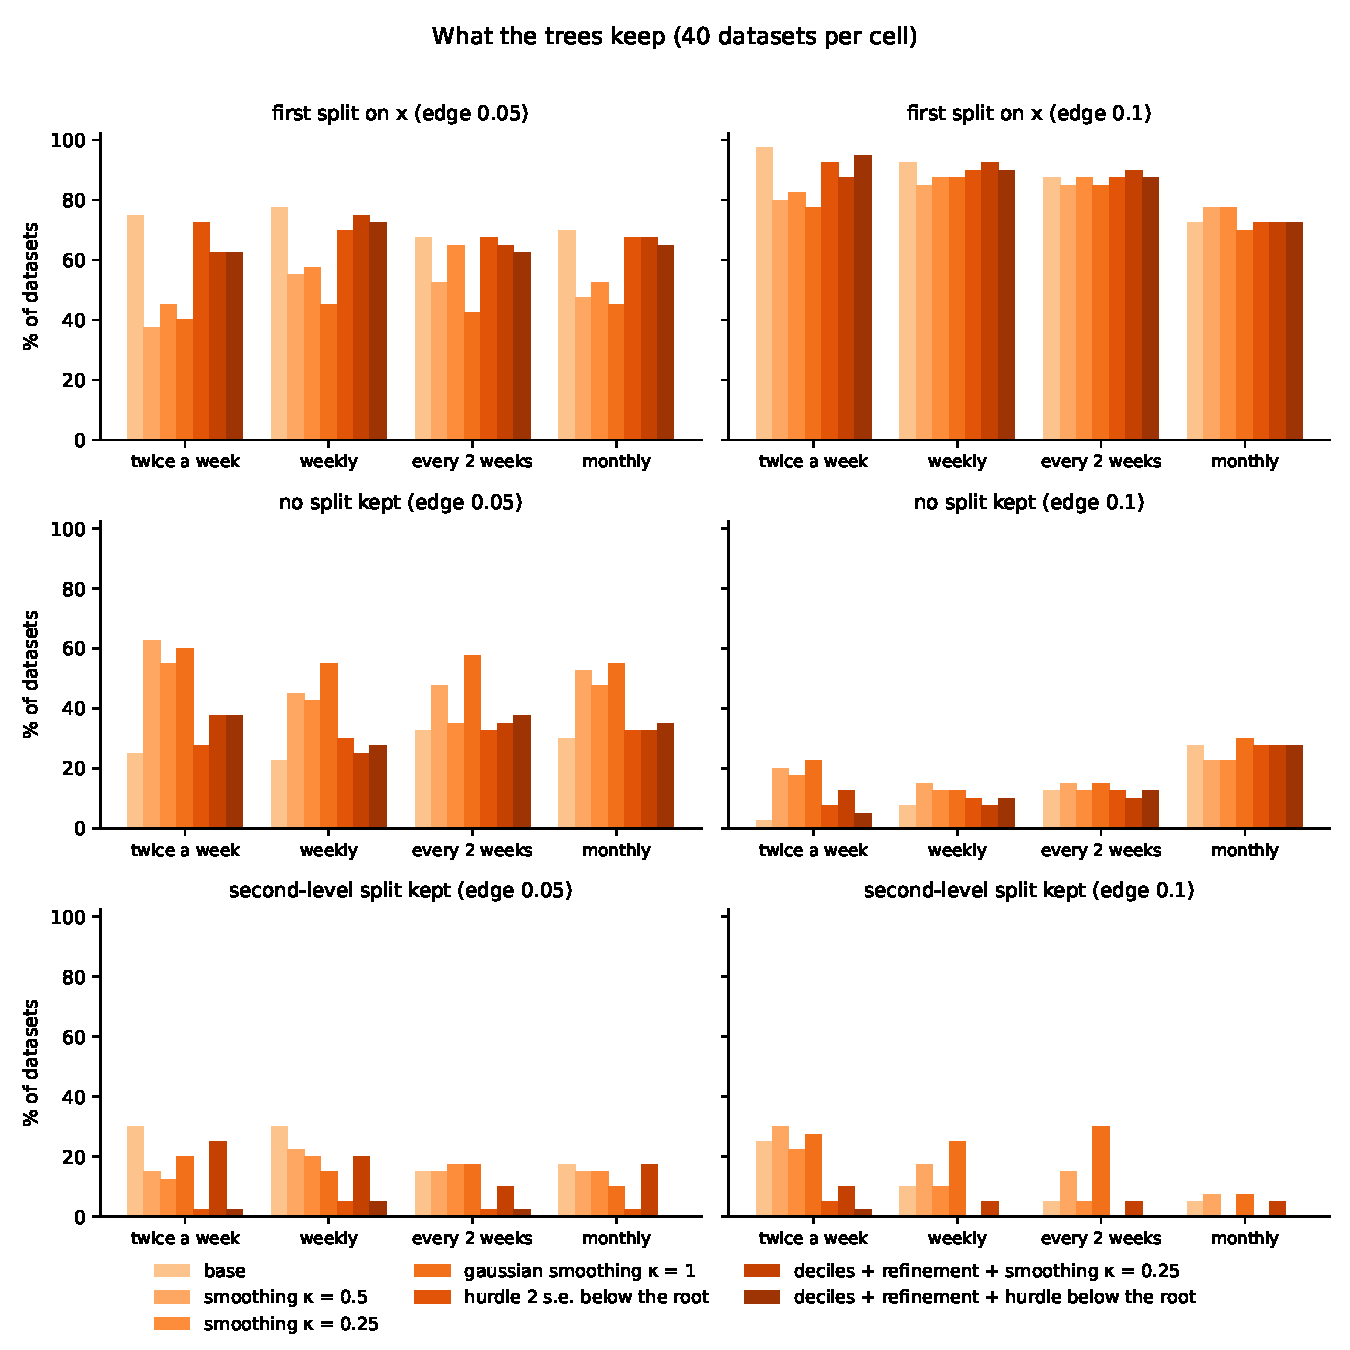
\includegraphics[width=\textwidth]{split_options_2_splits}
{\scriptsize Share of datasets with a first split on $x$, no split, and a second-level split, by option and rate (edge 0.10 left, 0.05 right).}
\column{0.56\textwidth}
\footnotesize
The pruning gain of a split is $\bar g$ over the checking rows; the hurdle asks $\bar g>k_p\,\mathrm{se}(\bar g)$.
\begin{itemize}
\item \bad{\textbf{Global hurdle}} ($k_p=1$ or 2 at every node): removes the spurious second-level leaves but loses true root splits, 60\% found at 2 s.e. against 98\% every 2 days, Sharpe 0.47 against 0.87. One quarter of the decisions (189 weekly) has not the power to confirm a real split at 2 s.e.
\item \good{\textbf{Hurdle 2 s.e. below the root}} (in v1): second-level splits fall from 25/10/5/5\% of the datasets to 5/0/0/0\% (2-day to monthly), the root is untouched, the Sharpe ratio is unchanged from weekly on (0.77, 0.68, 0.57 against 0.80, 0.69, 0.57), at edge 0.05 too.
\item Its cost: $-0.13$ every 2 days, where with 1{,}400 fitting decisions some second-level splits are real.
\end{itemize}
\end{columns}
\end{frame}

% ---------------------------------------------------------------------------------------------------
\begin{frame}{What can be found at all: resolution against volatility and noise (E6, 1{,}920 fits)}
\begin{center}
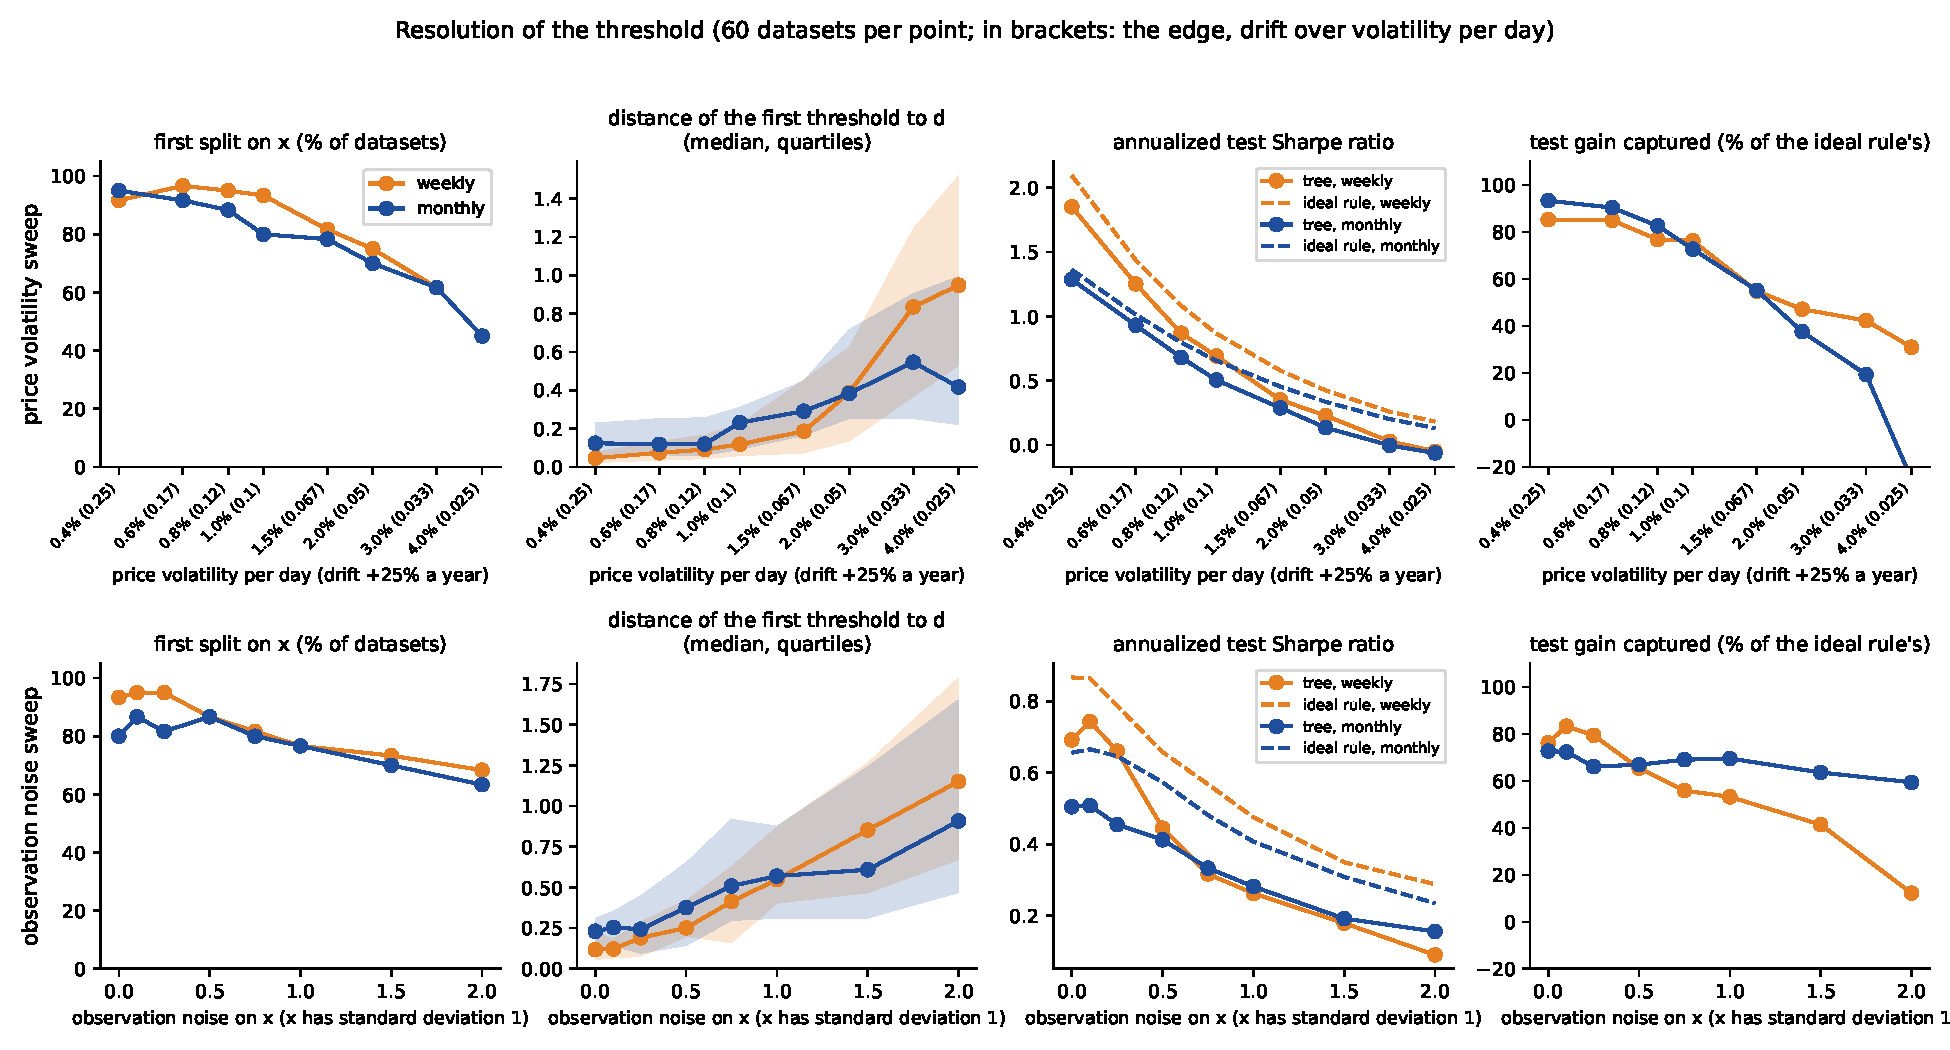
\includegraphics[width=0.68\textwidth]{resolution_curves}
\end{center}
\vspace{-4pt}\footnotesize
\begin{itemize}
\item Drift fixed at $\pm25\%$ a year, volatility swept: the threshold error is about $0.012/e$ standard deviations of $x$ until the edge falls below $0.05$, where the split becomes a guess (median $|\theta|$: 0.05 at $e=0.25$, 0.12 at 0.10, 0.39 at 0.05, 0.95 at 0.025).
\item White noise of $\tau$ standard deviations on the observed feature acts like dividing the edge by $1+\tau^2$: up to 0.25 costs nothing, 0.5 doubles the error, 1 halves the Sharpe of the ideal rule itself.
\item An edge below a few basis points a day will not be learnt from 15 years of data by any method: test a real feature with this protocol before trading it.
\end{itemize}
\end{frame}

% ---------------------------------------------------------------------------------------------------
\begin{frame}{A second market: the volatility follows a threshold too (E7, 2{,}240 fits)}\label{sl:regime}
\begin{columns}[T]
\column{0.36\textwidth}
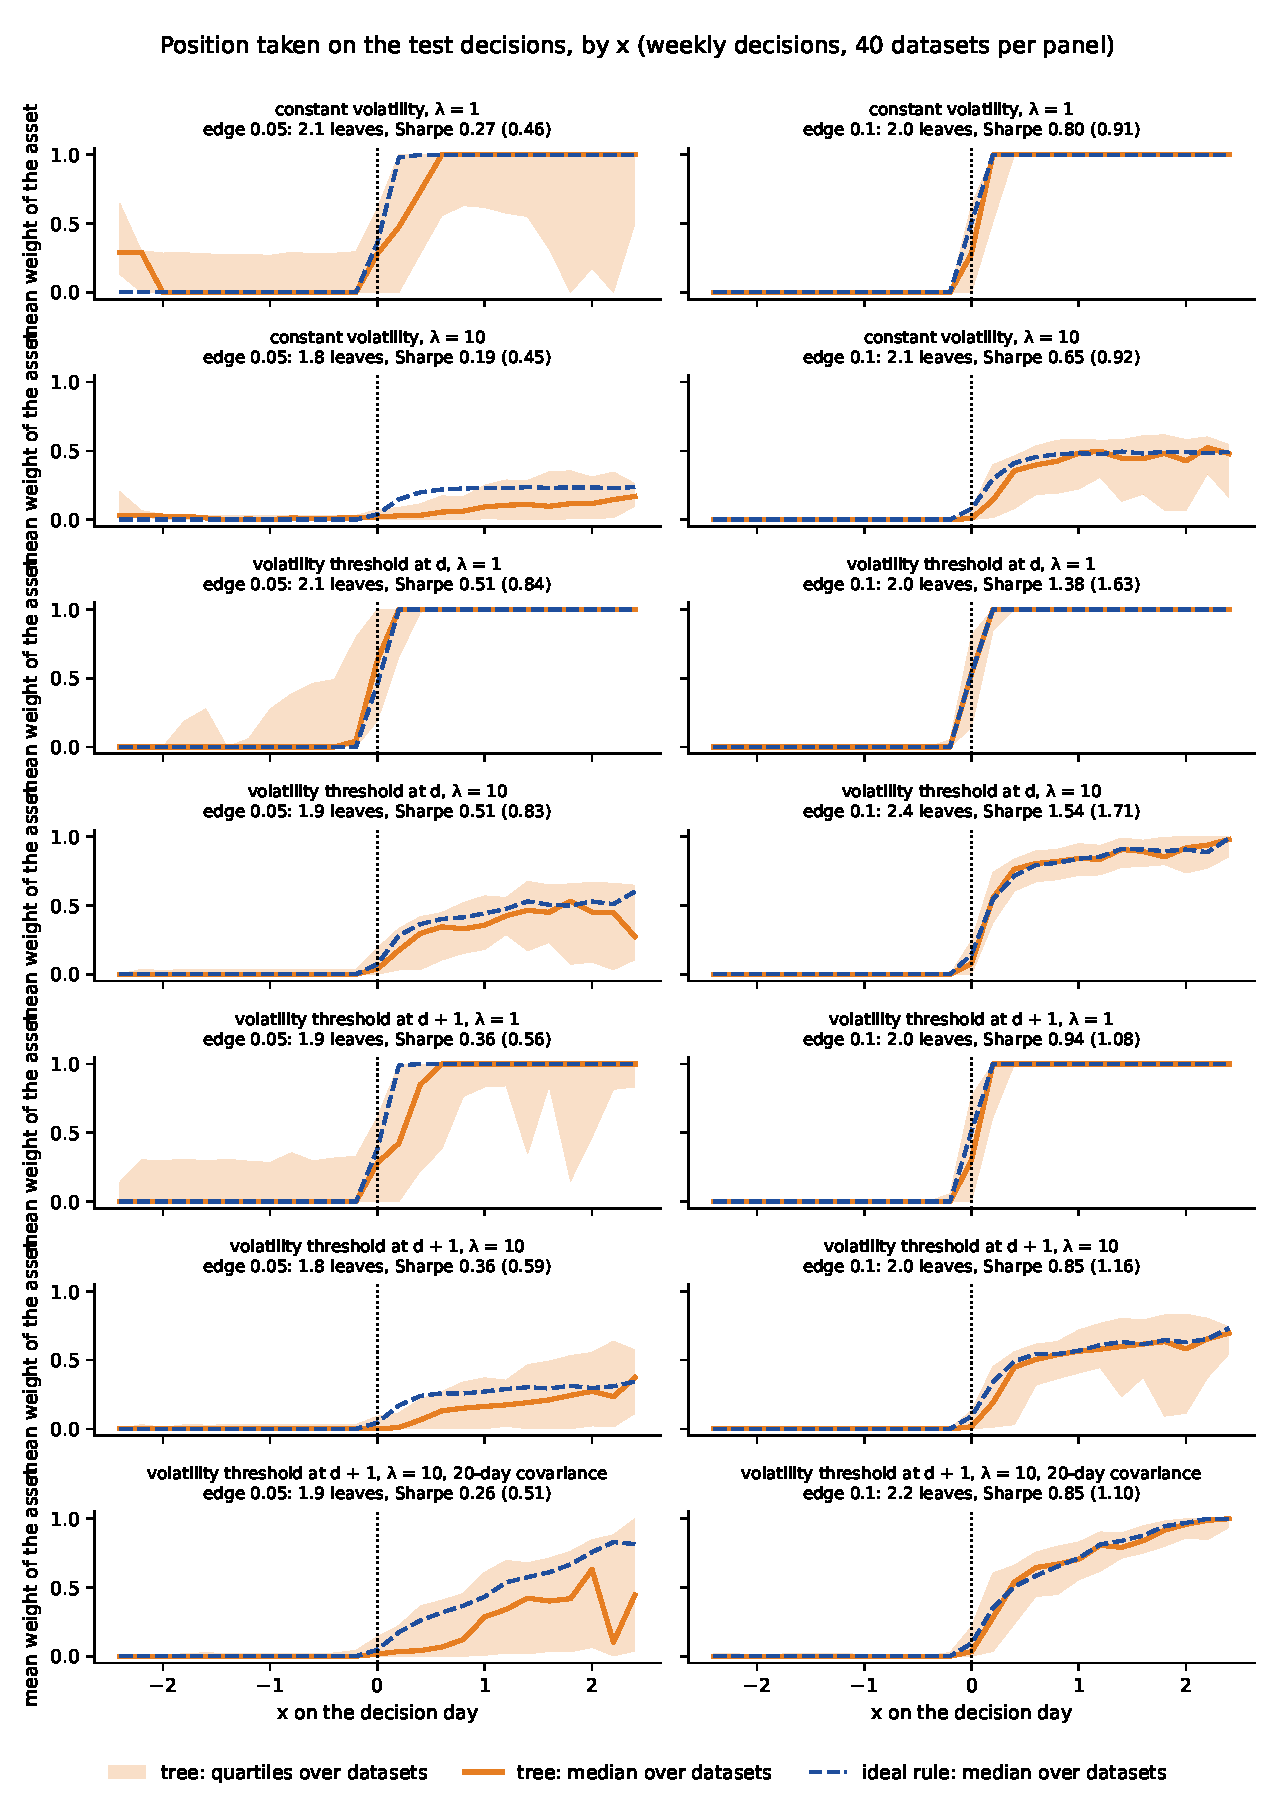
\includegraphics[height=0.84\textheight]{regime_volatility_positions}
\column{0.62\textwidth}
\footnotesize
$\sigma_t=0.5\%$ above $d_\sigma$, $1\%$ below; $d_\sigma=d$ (stress = bad regime) or $d_\sigma=d+1$ (a calm part inside the good regime, where the right position is \emph{smaller}, not of the other sign); $\lambda=1$ and $10$.
\begin{itemize}
\item \good{With $d_\sigma=d$ the drift threshold is found better}: within 0.25 of $d$ in 95\% of the weekly datasets (84\% with constant volatility); every Sharpe ratio nearly doubles; 83--86\% of the ideal gain kept. Clean returns in the good regime pin the threshold.
\item \bad{The volatility boundary at $d+1$ is not learnt}: 8--12\% of the trees split near $x=1$; calm-regime position 0.52 for the tree, 0.58 for the ideal rule on the same information, 0.96 for the clairvoyant rule.
\item Structural: the regret uses the same lagged 180-day covariance as the optimizer, which averages over regimes, so a boundary that exists only in the true variance has nothing to gain in the loss. \emph{The tree cannot learn what its own utility does not reward.}
\item A 20-day window follows the regime (calm position 0.69--0.75) but its noise costs more than the tracking gains. For v2: a regime-aware variance, not a deeper tree.
\end{itemize}
\end{columns}
\end{frame}

% ---------------------------------------------------------------------------------------------------
\begin{frame}{Model v1 on 100 datasets (E9, 800 fits), paired with the base of Result 1}\label{sl:v1}
\begin{columns}[T]
\column{0.58\textwidth}
\scriptsize\setlength{\tabcolsep}{3pt}
\begin{tabular}{@{}r r rr r r rr r@{}}
\toprule
& & \multicolumn{2}{c}{leaves} & 2nd level & within 0.25 & \multicolumn{2}{c}{Sharpe} & v1 $-$ base\\
\cmidrule(lr){3-4}\cmidrule(lr){7-8}
edge & $h$ & base & v1 & base $\to$ v1 & base $\to$ v1 & base & v1 & (2 s.e.)\\
\midrule
0.10 & 2 & 2.24 & 2.00 & 25 $\to$ 2\% & 92 $\to$ 89\% & 0.86 & 0.78 & $-0.08$ (0.07)\\
 & 5 & 2.14 & 1.94 & 18 $\to$ 0\% & 81 $\to$ 82\% & 0.73 & 0.73 & $+0.00$ (0.04)\\
 & 10 & 2.03 & 1.92 & 14 $\to$ 2\% & 70 $\to$ 72\% & 0.63 & 0.64 & $+0.01$ (0.05)\\
 & 21 & 1.90 & 1.81 & 9 $\to$ 0\% & 60 $\to$ 64\% & 0.54 & 0.53 & $-0.01$ (0.03)\\
\addlinespace
0.05 & 2 & 2.18 & 1.72 & 38 $\to$ 4\% & 64 $\to$ 57\% & 0.21 & 0.18 & $-0.03$ (0.06)\\
 & 5 & 2.01 & 1.80 & 21 $\to$ 3\% & 53 $\to$ 51\% & 0.24 & 0.22 & $-0.03$ (0.05)\\
 & 10 & 1.93 & 1.69 & 19 $\to$ 1\% & 47 $\to$ 49\% & 0.17 & 0.20 & $+0.03$ (0.04)\\
 & 21 & 1.76 & 1.59 & 13 $\to$ 0\% & 34 $\to$ 42\% & 0.17 & 0.14 & $-0.03$ (0.03)\\
\bottomrule
\end{tabular}

\smallskip\footnotesize
\begin{itemize}
\item \good{From weekly on, v1 is the base within noise}: second-level leaves gone, 1.9 leaves instead of 2.1, thresholds as well centred.
\item \bad{Every 2 days it costs $0.08\pm0.07$ at edge 0.10}: the hurdle removes second-level splits that are real there; the 2-day alternative needs a softer hurdle (not run).
\item The depth budget of 3 is never used here (at most 1\% of the trees reach the third level).
\item Verdict: \textbf{v1 is the base with a cleaner structure, not a higher Sharpe ratio.}
\end{itemize}
\column{0.4\textwidth}
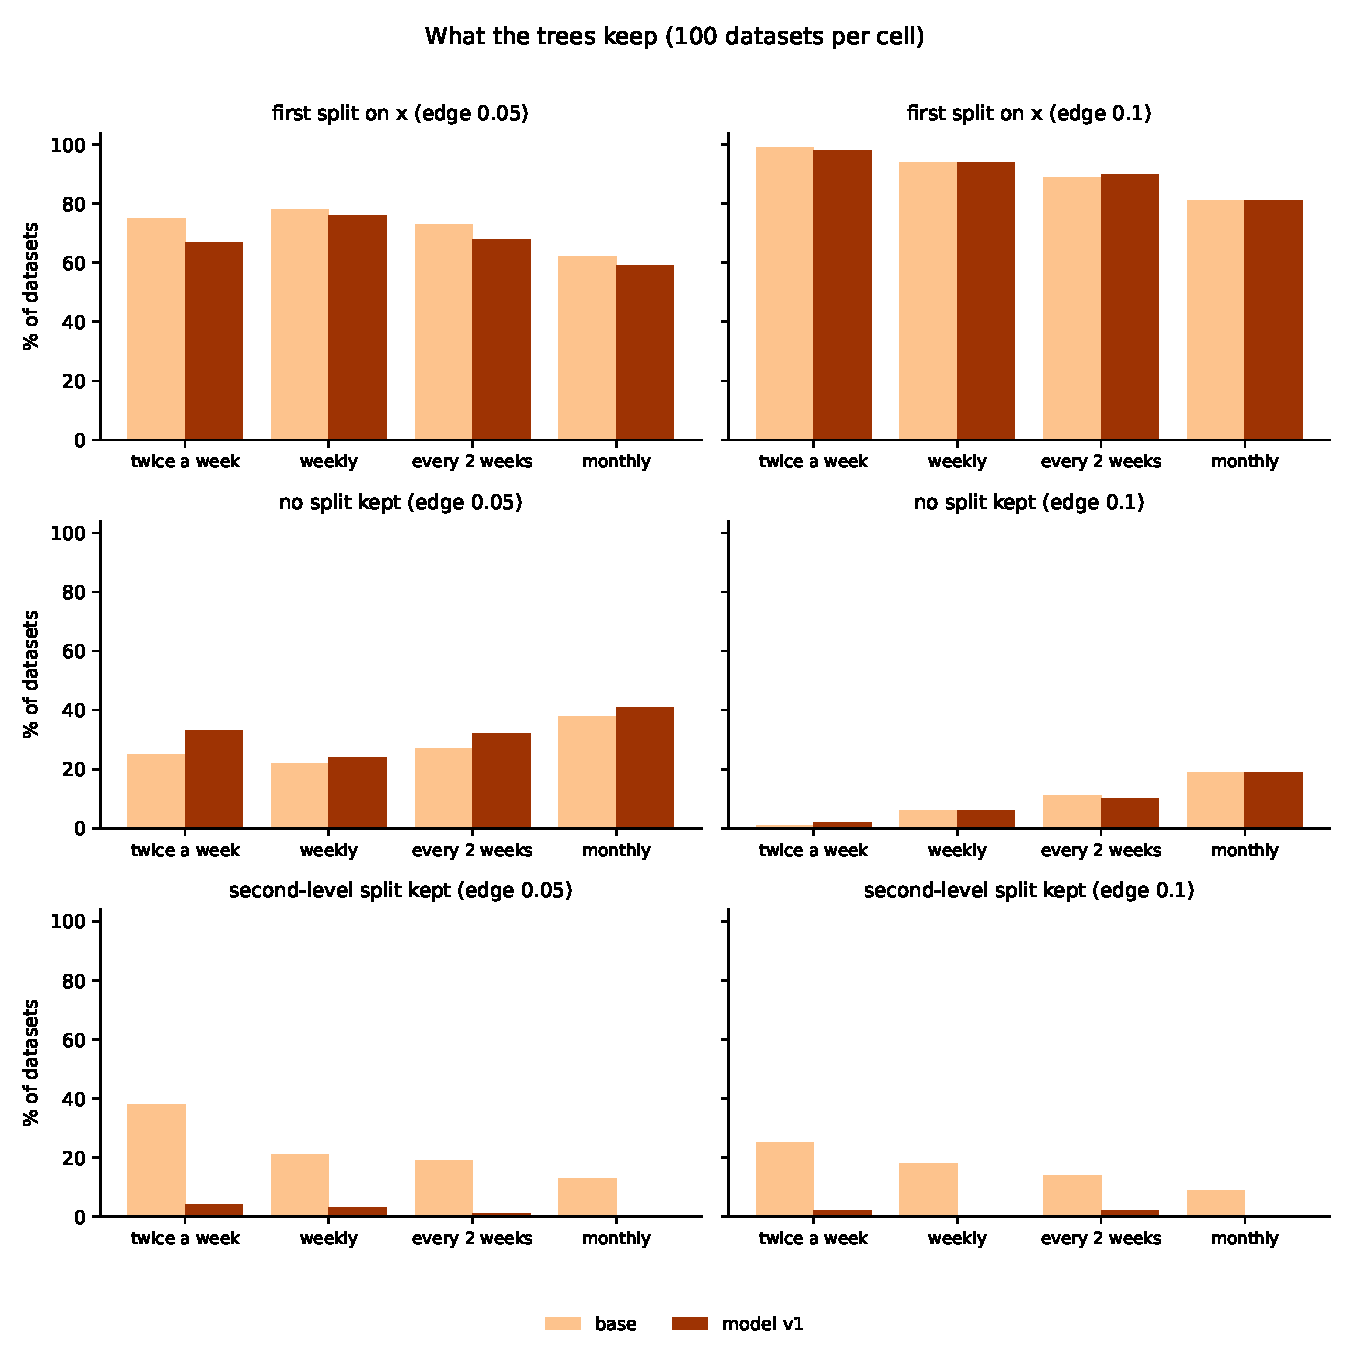
\includegraphics[width=0.92\textwidth]{model_v1_splits}

\scriptsize Same 100 datasets (seeds 0--99). ``2nd level'': datasets keeping a second-level split; ``within 0.25'': first threshold within 0.25 of $d$; last column: mean paired difference of annualized test Sharpe, twice its s.e.\ in brackets. In half of the datasets the two trees give the same Sharpe ratio.
\end{columns}
\end{frame}

% ---------------------------------------------------------------------------------------------------
\begin{frame}{A fair assessment}
\footnotesize
\begin{columns}[T]
\column{0.48\textwidth}
\begin{block}{What holds}
\begin{itemize}
\item The mechanism works at market sizes: a $\pm25\%$ regime on a monthly feature is recovered at every rate and 75--85\% of the attainable gain is earned out of sample; at $\pm13\%$ it degrades gracefully; at $\pm5\%$ it correctly finds nothing.
\item A regime that also drives the volatility is easier, not harder, when the calm regime is the profitable one.
\item The v1 additions (deciles + refinement, hurdle below the root) make the trees smaller and the thresholds steadier at no measurable cost from weekly on (100 paired datasets).
\item Everything is reproducible: results files, figures, dated history, 64 tests.
\end{itemize}
\end{block}
\column{0.5\textwidth}
\begin{block}{What is weak or untested}
\begin{itemize}
\item \textbf{No option beat the base beyond noise} (s.e. about 0.04 on 40 datasets), nor does v1 on 100. v1 buys stability, not Sharpe, and loses $0.08$ every 2 days.
\item \textbf{The growth gate on the replayed Sharpe is in-sample} and mixes a risk preference into the structure search; kept as designed, it is the first thing v2 tests (gate off, or the replayed regret instead).
\item \textbf{The pruning judge is one 25\% block}: too little power for a global hurdle; a split no checking row reaches cannot be confirmed.
\item \textbf{One clean feature.} Decoys were only tested at an unrealistic edge (0.95, E1); several features and interactions are untested at market sizes.
\item \textbf{Synthetic data only.} No real-data run, no neural benchmark.
\item \textbf{Approximate leaf search}; bang-bang positions at $\lambda=1$; volatility regimes invisible to the loss with a lagged covariance.
\end{itemize}
\end{block}
\end{columns}
\end{frame}

% ---------------------------------------------------------------------------------------------------
\begin{frame}{Next steps (towards v2)}
\begin{enumerate}
\item \textbf{The growth gate.} Run v1 with the Sharpe gate off, and with the path-replayed regret as the confirmation instead; same 100 datasets, paired.
\item \textbf{A regime-aware variance} for the optimizer and the regret (a variance driven by the feature, or an exponentially weighted estimate), then check that the second split appears at $d_\sigma$ in the regime market.
\item \textbf{Decoys and interactions at market sizes}: two features, four regimes, plus unrelated features; does the tree still ignore the decoys and find the interaction with a depth-3 budget?
\item \textbf{Feature denoising}: an exponentially weighted feature with the exact Gaussian-conditioned ideal rule as the ceiling (E6 says noise above 0.25 std matters).
\item \textbf{Position sizing}: $\lambda\ge5$ with soft splits, where smoothing the score does size the position.
\item \textbf{Real data} (the template \code{run_real_data.py}), with the planted-threshold protocol as the pre-test of every candidate feature; then the neural benchmark of the motivations note.
\end{enumerate}
\end{frame}

% ---------------------------------------------------------------------------------------------------
\begin{frame}{Appendix: the experiments behind the slides (\code{model_history.md})}
\scriptsize
\begin{tabular}{@{}l l l r p{7.6cm}@{}}
\toprule
id & date & market, pipeline & fits & headline\\
\midrule
E1 & 18 Sep & M1 (edge 0.95, 3 decoys), P1 & 800 & $x$ found first in 86--100\% of the datasets, never a decoy; drift far too large to be realistic\\
E2 & 22 Sep & M2, P2 (base) & 2{,}000 & threshold recovered at every rate at $\pm25\%$/yr, three times in four at $\pm13\%$, not at $\pm5\%$; monthly loses precision\\
E3 & 22 Sep & M2, P2 & 1{,}920 & depth alone changes nothing; $\lambda=5$--$10$ gives gradual positions at $-0.1$ Sharpe; 10 bp fees starve the fast rates\\
E4 & 23 Sep & M2, P3b & 1{,}600 & deciles + refinement $\approx$ base with steadier thresholds; smoothing $\kappa=1$ too wide, inside the no-trade band\\
E5 & 23 Sep & M2, P3b & 1{,}600 & a global pruning hurdle removes spurious leaves but loses true root splits\\
E6 & 23 Sep & M2$'$ (noise), P3b & 1{,}920 & threshold error $\approx0.012/e$ until $e\approx0.05$; noise $\tau$ acts like edge$/(1+\tau^2)$\\
E7 & 23 Sep & M2$'$ (regime volatility), P3b & 2{,}240 & drift threshold found better with $d_\sigma=d$; the volatility boundary is not learnt (lagged covariance)\\
E8 & 23 Sep & M2, P4 & 2{,}240 & $\kappa=0.25$ cures the no-trade problem, still $-0.26$ at 2 days; hurdle below the root removes second-level leaves at no cost from weekly on\\
E9 & 24 Sep & M2, P4 in configuration v1 & 800 & v1 = base within noise from weekly on ($0.00\pm0.04$ weekly at edge 0.10), second-level leaves gone; $-0.08\pm0.07$ every 2 days (slide~\ref{sl:v1})\\
\bottomrule
\end{tabular}

\medskip
Pipelines: P1 first tree (18 Sep), P2 all-cash Sharpe $=0$ (22 Sep), P3/P3b split-search options and rank quantiles (23 Sep), P4 Gaussian kernel and depth-restricted hurdle (23 Sep evening). Markets: M1 the first world, M2 the daily market with the threshold at the mean, M2$'$ with observation noise and regime volatility as options. Reproduce: \code{python planted_threshold_experiments.py run | run-settings | run-enhancements | run-pruning | run-resolution | run-regime | run-options | run-v1 | plot} from \code{code/}.
\end{frame}

\end{document}
